%%%%%%%%%%%%%%%%%%%%%%%%%%%%%%%%%%%%%%%%%%%%%%%%%%%%%%%%%%%%%%%%%%%%%%
% LaTeX Example: Project Report
%
% Source: http://www.howtotex.com
%
% Feel free to distribute this example, but please keep the referral
% to howtotex.com
% Date: March 2011 
% 
%%%%%%%%%%%%%%%%%%%%%%%%%%%%%%%%%%%%%%%%%%%%%%%%%%%%%%%%%%%%%%%%%%%%%%
% How to use writeLaTeX: 
%
% You edit the source code here on the left, and the preview on the
% right shows you the result within a few seconds.
%
% Bookmark this page and share the URL with your co-authors. They can
% edit at the same time!
%
% You can upload figures, bibliographies, custom classes and
% styles using the files menu.
%
% If you're new to LaTeX, the wikibook is a great place to start:
% http://en.wikibooks.org/wiki/LaTeX
%
%%%%%%%%%%%%%%%%%%%%%%%%%%%%%%%%%%%%%%%%%%%%%%%%%%%%%%%%%%%%%%%%%%%%%%
% Edit the title below to update the display in My Documents
%\title{Project Report}
%
%%% Preamble
\documentclass[paper=letter, fontsize=10pt]{scrartcl}
\usepackage[body={7in,7.5in},top=1in, bottom=1in]{geometry}
\usepackage[T1]{fontenc}
\usepackage{fourier}

\usepackage[english]{babel}															% English language/hyphenation
\usepackage[protrusion=true,expansion=true]{microtype}	
\usepackage{amsmath,amsfonts,amsthm} % Math packages
\usepackage[pdftex]{graphicx}	
\usepackage{url}
\usepackage{enumerate}
\usepackage{lastpage}


%%% Custom sectioning
\usepackage{sectsty}
\allsectionsfont{\normalfont\scshape}


%%% Custom headers/footers (fancyhdr package)
\usepackage{fancyhdr}
\pagestyle{fancy}
\fancyhead[L]{}
\fancyhead[c]{User Manual Revision 1}
\fancyhead[R]{\today}											
\fancyfoot[L]{}											 
\fancyfoot[C]{}											
\fancyfoot[R]{\thepage\ of \pageref{LastPage}}		% Pagenumbering
\renewcommand{\headrulewidth}{0.4pt}				% Remove header underlines
\renewcommand{\footrulewidth}{0.4pt}				% Remove footer underlines
\setlength{\headheight}{13.6pt}


%%% Equation and float numbering
\numberwithin{equation}{section}		% Equationnumbering: section.eq#
\numberwithin{figure}{section}			% Figurenumbering: section.fig#
\numberwithin{table}{section}				% Tablenumbering: section.tab#


%%% Maketitle metadata
\newcommand{\horrule}[1]{\rule{\linewidth}{#1}} 	% Horizontal rule
\newcommand{\ts}{\textsuperscript}

%%% Begin document
\begin{document}

\begin{titlepage}

\newcommand{\HRule}{\rule{\linewidth}{0.5mm}} % Defines a new command for the horizontal lines, change thickness here

\begin{center}
 
%----------------------------------------------------------------------------------------
%	HEADING SECTIONS
%----------------------------------------------------------------------------------------

\textsc{\LARGE McMaster University}\\[1.5cm] % Name of your university/college
\textsc{\Large CAS 4ZP6 Capstone Project 2013/2014}\\[0.5cm] % Major heading such as course name
\textsc{\large Porter Simulation}\\[0.5cm] % Minor heading such as course title

%----------------------------------------------------------------------------------------
%	TITLE SECTION
%----------------------------------------------------------------------------------------

\HRule \\[0.4cm]
{ \huge \bfseries User Manual Revision 1}\\[0.4cm] % Title of your document
\HRule \\[1.5cm]
 
%----------------------------------------------------------------------------------------
%	AUTHOR SECTION
%----------------------------------------------------------------------------------------

\begin{minipage}{0.4\textwidth}
\begin{flushleft} \large
\emph{Authors:}\\
Vitaliy Kondratiev - 0945220\\
Nathan Johrendt - 0950519\\
Tyler Lyn - 0948978\\
Mark Gammie - 0964156
\end{flushleft}
\end{minipage}
~
\begin{minipage}{0.4\textwidth}
\begin{flushright} \large
\emph{Supervisor:} \\
Dr. Douglas Down % Supervisor's Name
\end{flushright}
\end{minipage}\\[4cm]

% If you don't want a supervisor, uncomment the two lines below and remove the section above
%\Large \emph{Author:}\\
%John \textsc{Smith}\\[3cm] % Your name

%----------------------------------------------------------------------------------------
%	DATE SECTION
%----------------------------------------------------------------------------------------

{\large \today}\\[3cm] % Date, change the \today to a set date if you want to be precise

%----------------------------------------------------------------------------------------
%	LOGO SECTION
%----------------------------------------------------------------------------------------

%\includegraphics{Logo}\\[1cm] % Include a department/university logo - this will require the graphicx package
 
%----------------------------------------------------------------------------------------

\vfill % Fill the rest of the page with whitespace
\end{center}
\end{titlepage}

\setcounter{tocdepth}{2}

\tableofcontents

\newpage
\section{Introduction}
Welcome to the User Manual for the Hamilton Health Science's Porter Simulation, designed for use at the Juravinski Hospital in Hamilton, Ontario. This manual will examine the topics of installation, input configuration, running the simulation, output data and configuring the development environment.  This manual will also explain to the reader the meaning of each option in the User Interface and provide the reader with background information.

\section{Background}
This section provides the reader with a high-level overview of key components within the simulation.  The simulation begins by importing all of the settings configured through the software's user interface.  A data file containing all information about jobs will be sampled by the software and a list of jobs will be generated.  The sampling of this data file can be configured through the Basic Settings (Section 5.1).  Jobs will then be passed into the Dispatcher and assigned to porters.  The Dispatcher can be configured through the Advanced Settings (Section 5.3).  Once the simulation is finished an excel file is generated allowing the user to view raw simulation data and graphs (Section 6).
	
\section{Installation}
Setup of the Porter Simulation will be done by running an installer.
\begin{enumerate}
	\item Locate the Porter Simulation-1.0-win32.exe file.
	\item Double click to run the Porter Simulation-1.0-win32.msi
	\item Pick a directory to install the application. Default directory will be automatically filled in
	\item Wait for the installer to finish then click "Finish"
	\item The Porter Simulation shortcut will now appear on your desktop
\end{enumerate}

\begin{figure}[!htbp]
	\begin{center}
		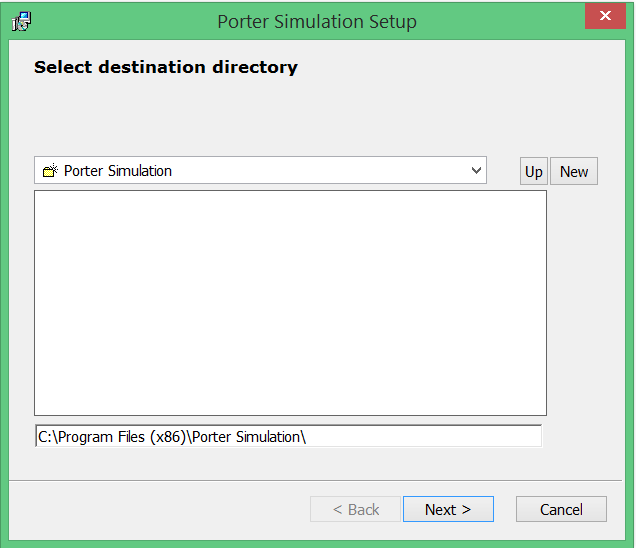
\includegraphics[width=1\columnwidth, height=0.3\textheight, keepaspectratio]{Installer.png}
		\caption{Pick a directory}
	\end{center}
\end{figure} 

	\subsection{Generate Installation File}
	Before building Porter Simulation-1.0-win32.exe the reader must have a working development environment (Section 8: Configure Development Environment)
	\begin{enumerate}[(i)]
		\item From command prompt enter: \textbf{python setup.py bdst\_msi}
		\item Two folders named "build" and "dist" will be generated
		\item The build folder contains an executable to run the simulation
		\item The dist folder contains the installer (i.e. Simulation-1.0-win32.exe) 	
	\end{enumerate}

\section{Launch Simulation Tool}
The Porter Simulation tool can be launched by double-clicking on the PorterSimulation2014.exe

\section{Input Configuration}
The first step in using the software is to configure the simulation with a series of different inputs. These different input variables represent changes to the hospital environment, which will affect the simulated results.

	\begin{figure}[!htbp]
	\begin{center}
		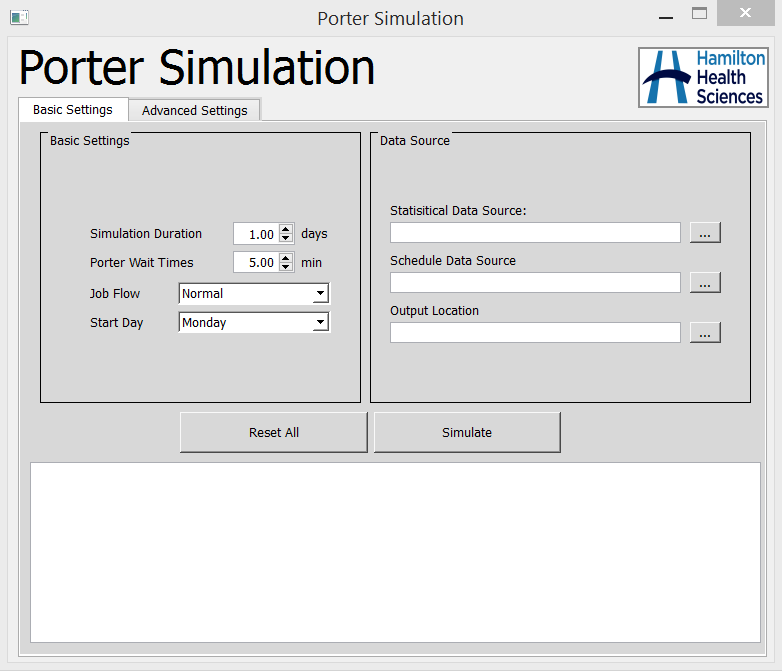
\includegraphics[width=1\columnwidth, height=0.45\textheight, keepaspectratio]{BasicSettings.png}
		\caption{Basic Settings}
	\end{center}
	\end{figure} 
	\subsection{Basic Settings}
	\begin{enumerate}[(i)]
		\item \textbf{Simulation Duration:} Number of days the software will simulate events. Minimum: 1 Maximum: 7
		\item \textbf{Porter Wait Times:} Maximum number of minutes a porter waits for a delay (patient, equipment, nurse) before cancelling a job
		\item \textbf{Job Flow:} The rate of event generation during the course of the simulation. The levels are Low, Normal, High. On normal the rate of job creation is consistent to how it appears in the data. On Low and High level the rate is decreased and increased respectively 
		\item \textbf{Start Day:} Define the first day the simulation generates events from. For example; specifying Tuesday means day 1 events will only come from Tuesdays of the statistical data source, day 2 events will come from Wednesday, etc.
	\end{enumerate}
	
	\subsection{Basic Settings - Data Source}
	The Data Source setting allows selection of different source input files, pre-configured to aid HHS users in testing a variety of hospital conditions and elements. 
	\begin{enumerate}[(i)]
		\item \textbf{Statistical Data Source:} A path to the source file that will be used to provide the simulation with statistical distribution information. For more information see section 5.5
		\item \textbf{Schedule Data Source:} A path to the source file that will be used to provide scheduling information to be used during simulation. For more information see section 5.4
		\item \textbf{Output Location:} Determines the Location to store output data
	\end{enumerate}
	
	\subsection{Advanced Settings}
	The dispatcher will be ordering the pending jobs and giving them to available porters.  The dispatcher algorithm was designed using documentation provided by HHS.  The values for Appointment Factor, Automatic Job Priority Values and Weighted Job List are set to the default values provided in the documentation.
	
	\begin{figure}[!htbp]
	\begin{center}
		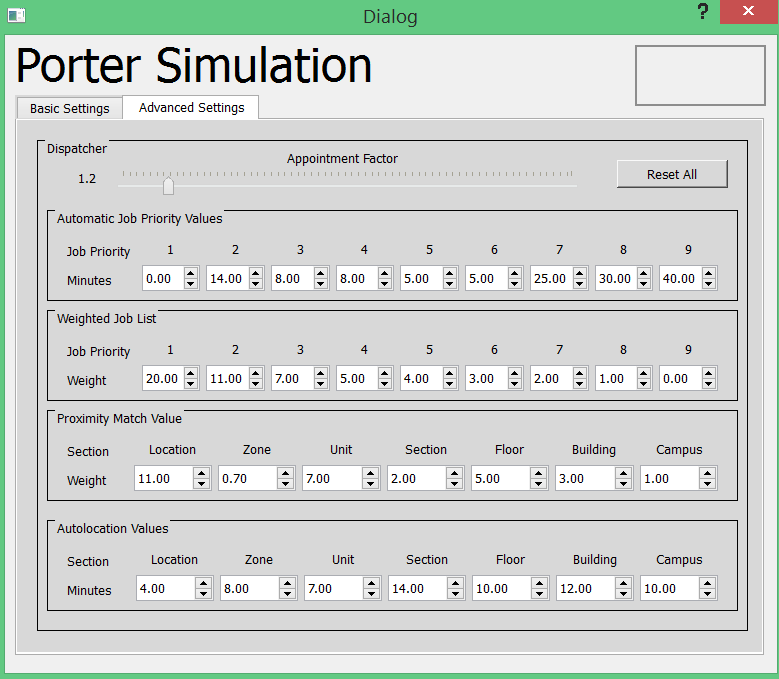
\includegraphics[width=1\columnwidth, height=0.45\textheight, keepaspectratio]{AdvancedSettings.png}
		\caption{Advanced Settings}
	\end{center}
	\end{figure} 
	\begin{enumerate}[(i)]
		\item \textbf{Appointment Factor:} Jobs that are scheduled in advance need to be given priority over jobs generated on-demand.  Increasing the appointment factor will decrease the time scheduled jobs spend waiting for a porter.
		\item \textbf{Automatic Job Priority Values:} Jobs waiting for a porter need to increase their priority after waiting for a specified amount of time.  The "Minutes" will determine how long a job waits until it increases in priority.
		\item \textbf{Weighted Job List:} Jobs of different priorities need to have different weights.  This weight helps determine how quickly the job should be assigned to a porter.
		\item \textbf{Random Seed:} Gives the user the ability to specify a random seed variable. Specific seeds will give unique output data linked to that seed. Setting this value to 0 will make the simulation choose a random seed during runtime. Every simulation exists with the seed used. Record your seed after running a random seed simulation to get the exact same results
		\begin{figure}[!htbp]		
		\begin{center}
			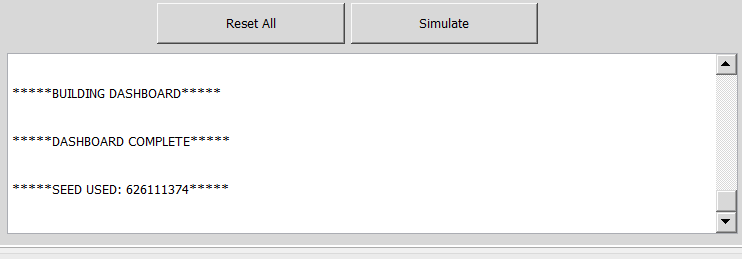
\includegraphics[width=1\columnwidth, height=0.45\textheight, keepaspectratio]{randomSeed.png}
			\caption{Random Seed}
		\end{center}
		\end{figure} 
	\end{enumerate}
	
	\subsection{Porter Schedule}
	Porters need to be scheduled by shifts in order to give the users flexibility over the simulation.  This will allow the user full control over the amount of porters available over the course of a simulation.
	
	\begin{figure}[!htbp]
	\begin{center}
		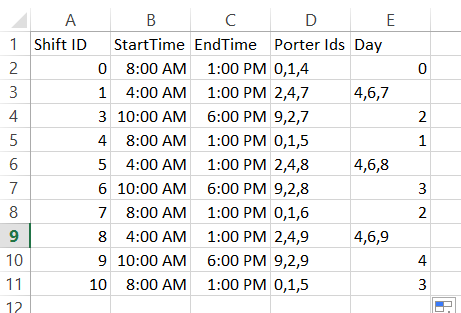
\includegraphics[width=1\columnwidth, height=0.5\textheight, keepaspectratio]{Schedule.png}
		\caption{Porter Schedule}
	\end{center}
	\end{figure}
	
	\begin{enumerate}[(i)]
		\item \textbf{Shift ID:} An identifier for a shift.  The Shift ID will allow for easier traceability of shifts in the output data.
		\item \textbf{StartTime:} A shift will begin at this time in the simulation.
		\item \textbf{EndTime:} A shift will end at this time in the simulation.
		\item \textbf{Porters Ids:} Allows for the assignment of one or more porter(s) to a shift.  A porter is assigned to a shift by adding an identifier.  Multiple porters can be assigned to the same shift by adding multiple identifiers each separated by a comma.  In the Figure 5.4 \textit{Shift ID 0} has three  porters assigned to it \textit{0,1,2,3,4,5,6}.
		\item \textbf{Day:} The day of the week on which the shift occurs.  It must be a number from 1-7, 1 being day 1 as specified by Start Day and 7 being day 7.
	\end{enumerate}

	\subsection{Statistical Data Source}
	The data source is the direct output used by HHS during operations. This file must be of the same format for the simulation to function properly. Fields include (in order; * is a required field)
	\begin{enumerate}
	\item \textbf{TransportJobID}
	\item \textbf{SequenceOrder}
	\item \textbf{Campus}
	\item \textbf{Last\_Status*}
	\item \textbf{StatusDate}
	\item \textbf{Requester}
	\item \textbf{Origin*}
	\item \textbf{Destination*}
	\item \textbf{JobPriorityID}
	\item \textbf{OriginalPriorityID*}
	\item \textbf{Transporter}
	\item \textbf{AppointmentDT}
	\item \textbf{PendingDT*}
	\item \textbf{DispatchedDT*}
	\item \textbf{InProgressDT*}
	\item \textbf{CompleteDT*}
	\item \textbf{DelayMin*}
	\item \textbf{DelayReason*}
	\item \textbf{DispatchMins (PE-DI)}
	\item \textbf{ResponseMins (PE-IP)}
	\item \textbf{ArrivalMins (DI-IP)}
	\item \textbf{TransactionMins (PE-CO)}
	\item \textbf{TripMins (DI-CO)}
	\item \textbf{PatientMins (IP-CO)}
	\item \textbf{LostPorterMinsOnCancel (DI-CA)}
	\item \textbf{PatientTransportFlag*}
	\item \textbf{PendWeekendFlag}
	\item \textbf{Created\_Status*}
	\item \textbf{RequesterType}
	\item \textbf{OriginZone}
	\item \textbf{OriginBuilding}
	\item \textbf{OriginUnit}
	\item \textbf{DestinZone}
	\item \textbf{DestinBuilding}
	\item \textbf{DestinUnit}
	\item \textbf{NumberOfJobsBatched}
	\item \textbf{BatchedToJobID}
	\item \textbf{ModeOfTravel}
	\item \textbf{TotalTransportersRequired}
	\item \textbf{TransportItem}	
	\item \textbf{ReasonCodeID}
	\item \textbf{NumberOfPages}
	\item \textbf{UniqueTransportJobID}
	\item \textbf{RejectCount}
	\end{enumerate}
	
\newpage
\section{Dashboard}
Once the simulation has finished, the results of all of the completed jobs are exported to an excel file. The file is located at the directory specified at the configurable \textbf{Output Location}. Upon opening the file please enable macros as specified by your version of Microsoft Excel. Once macros have been enabled click the "Recalculate" button on any of the Sheets named "Dashboard D(1-7)" to calculate the statistics and update all the graphs. Each tab represents data for one day of simulation broken up into 18 time intervals.

	\begin{figure}[!htbp]
	\begin{center}
		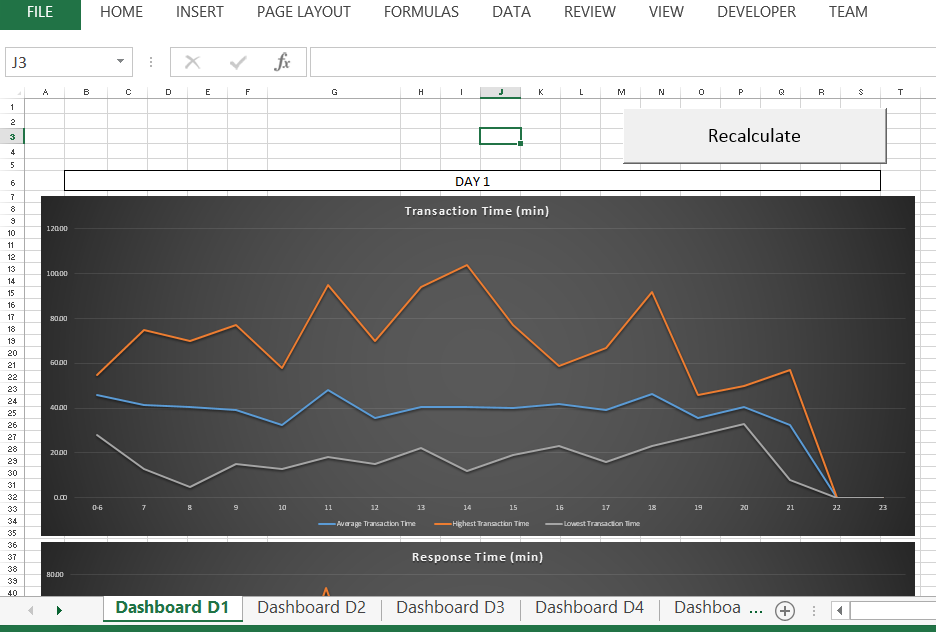
\includegraphics[width=1\columnwidth, height=0.4\textheight, keepaspectratio]{Dashboard.png}
		\caption{Dashboard}
	\end{center}
	\end{figure}
	
		\begin{figure}[!htbp]
		\begin{center}
			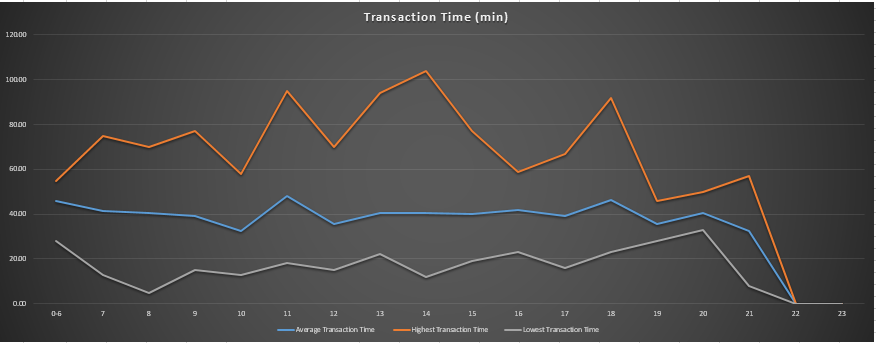
\includegraphics[width=1\columnwidth, height=0.3\textheight, keepaspectratio]{transactionTime.png}
			\caption{\textbf{Transaction Time:} Represents the transaction time for a job created in a specific time interval. Transaction time is defined as the time from when a job is created to when a job has been complete. Chart contains High, Low and Average values.}
		\vspace{-5em}
		\end{center}
		\end{figure}
		
		\begin{figure}[!htbp]		
		\begin{center}
			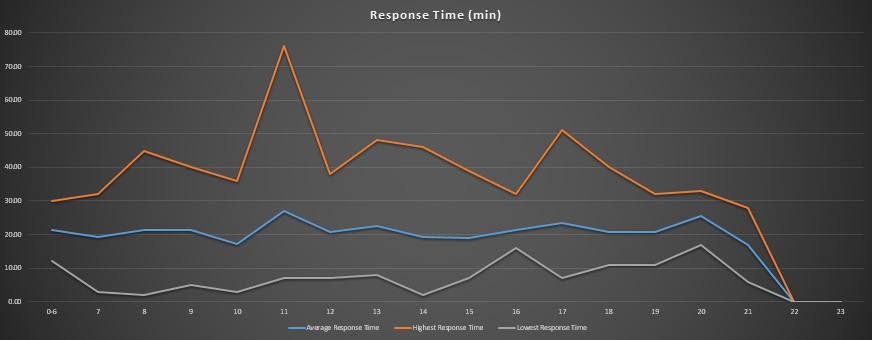
\includegraphics[width=1\columnwidth, height=0.4\textheight, keepaspectratio]{responseTime.png}
			\caption{\textbf{Response Time:} Represents the response time for a job created in a specific time interval. Response time is defined as the time from when a job has been created to when a job has been taken on by a porter. Chart contains High, Low and Average values.}
		\end{center}
		\end{figure}
		\begin{figure}[!htbp]		
		\begin{center}
			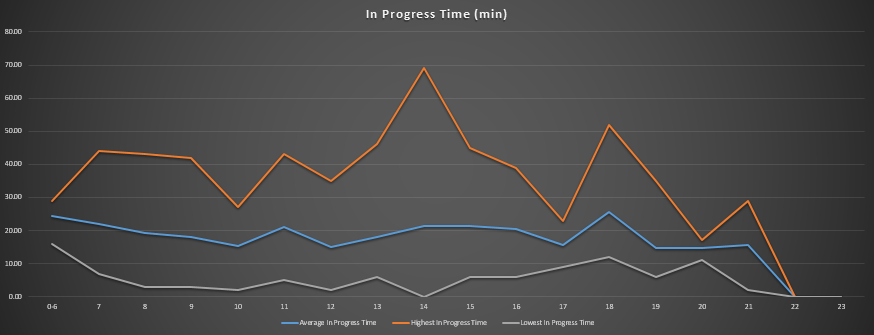
\includegraphics[width=1\columnwidth, height=0.4\textheight, keepaspectratio]{inProgress.png}
			\caption{\textbf{In Progress Time:} Represents the in progress time for a job created in a specific time interval. In progress time is defined as the time from when a job has been taken on by a porter to when a job has been complete. Chart contains High, Low and Average values.}
		\end{center}
		\end{figure}
		\begin{figure}[!htbp]		
		\begin{center}
			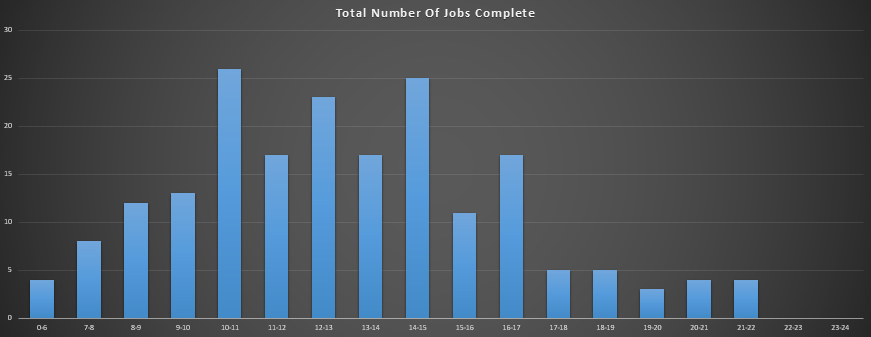
\includegraphics[width=1\columnwidth, height=0.4\textheight, keepaspectratio]{numberOfJobs.png}
			\caption{\textbf{Job Distribution:} This graph shows the Number of Jobs created/completed/responded to in the time interval.}
		\end{center}
		\end{figure}
		\begin{figure}[!htbp]		
		\begin{center}
			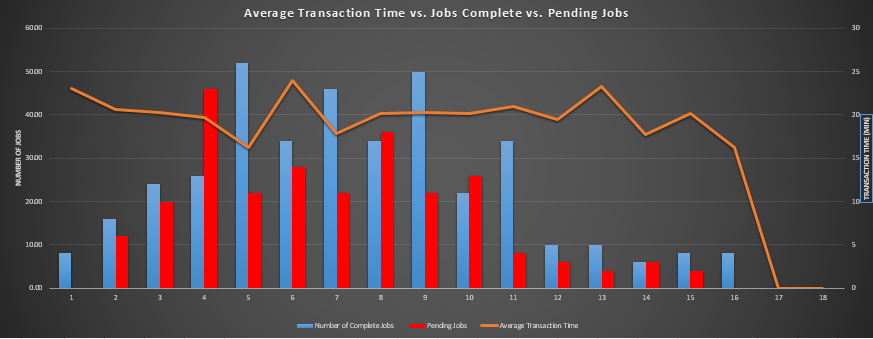
\includegraphics[width=1\columnwidth, height=0.4\textheight, keepaspectratio]{comboChart.png}
			\caption{\textbf{Average Transaction Time vs. Jobs Complete vs. Pending Jobs:} Pending Jobs represent any jobs that are still active at the end of each time interval. Number of Complete Jobs and Average Transaction Times are overlaid here.}
		\end{center}
		\end{figure}
		\begin{figure}[!htbp]		
		\begin{center}
			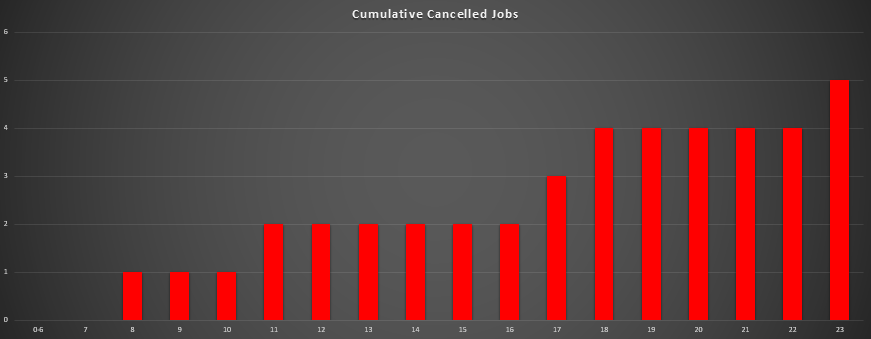
\includegraphics[width=1\columnwidth, height=0.4\textheight, keepaspectratio]{cancelledJobs.png}
			\caption{\textbf{Cumulative Cancelled Jobs:} Represents the total number of cancelled jobs for at the end of each time interval}
		\end{center}
		\end{figure}
	
\section{Raw Data}
Raw data can be accessed from the generated dashboard files. Simply right click on any of the bottom tabs and pick the unhide option. Each dashboard has a corresponding data sheet. All the raw events data is in Sheet1. 


\section{Configure Development Environment}
These instructions are for setting up a development environment for running and editing the source code.  The following instructions were made for Microsoft Windows 7 operating system.

\subsection{Install Python Modules}
\begin{enumerate}[(i)]
	\item Visit https://www.python.org/download/releases/2.7.6 and download run the "Windows x86 MSI Installer (2.7.6)".
	\item After Python is installed add the python path (i.e. C:\textbackslash{Python27}) to the Windows System Variables.
	\item Download the pip installation file from http://www.pip-installer.org/en/latest/installing.html and install it using the cmd: \textbf{python get-pip.py}
	\item After pip has been downloaded and installed add the path (i.e. C:\textbackslash{Python27}\textbackslash{Scripts}) to the Windows System Variables
	\item Download the binary installer for PyQT 4 and run the executable: http://www.riverbankcomputing.com/software/pyqt/download
	\item With command prompt run: \textbf{pip install python-dateutil}
	\item With command prompt run: \textbf{pip install simpy}
	\item With command prompt run: \textbf{pip install xlst}
	\item Download the installer for pywin32 and run the executable: http://sourceforge.net/projects/pywin32/files/pywin32/Build\%20218/
	\item Download the installer for cx\_freeze and run the msi: http://cx-freeze.sourceforge.net/
	\item Ensure you have a copy of Microsoft Excel (version 2010 or higher) installed on the system to view the dashboard generated file 
\end{enumerate}

\section{Troubleshooting}
The troubleshooting section should be used to help address minor issues that may arise.

\begin{enumerate}[(i)]
	\item \textbf{Missing Files and Locations:} Failing to specify the correct locations of required files will result in program halts
	\item \textbf{Incorrect Schedule Data:} In the event of incorrect schedule input, the program will halt and alert you with the location of the error
	\item \textbf{Simulation Stops:} In the event that the simulation is running and suddenly halts before producing output data, it will be necessary to close the simulation manually by clicking the X in the top right corner of the window. If the simulation continues to malfunction, please contact the development team.
\end{enumerate}

\section{Figures and Tables Appendix}
\begin{itemize}
	\item Figure 3.1: Installer (Page 3)
	\item Figure 5.1: BasicSettings (Page 4)
	\item Figure 5.3: AdvancedSettings.png (Page 5)
	\item Figure 5.4: Schedule.png (Page 6)
	\item Figure 6.1: Dashboard Overview (Page 7)
	\item Figure 6.2: Transaction Time (Page 7)
	\item Figure 6.3: Response Time (Page 8)
	\item Figure 6.4: In Progress Time (Page 8)
	\item Figure 6.5: Total Number of Jobs Complete (Page 9)
	\item Figure 6.6: Comparison Graph (Page 9)
	\item Figure 6.7: Cumulative Cancelled Jobs (Page 10)
\end{itemize}

\section{Legal and Copyright Information}
Ownership of software and accompanying documentation developed at McMaster University by the Porter Simulation project team is covered by the Joint Intellectual Property Policy as well as the Ownership of Student Work Policy. This software and accompanying documentation is licensed freely for access by Hamilton Health Sciences staff, project supervisor Dr. Douglas Down, and the Comp Sci 4ZP6 course instructors.

\section{Contact Information}
The Development team can be contacted for praise or support at kondrav@live.ca.



%%% End document	
\end{document}	